
%
%   trk_performance.tex
%       author: Omar Moreno <omoreno1@ucsc.edu>
%      created: December 4, 2012
%
 
A charged particle traversing the sensitive volume of the SVT is expected to
deposit enough charge to produce hits which, in turn, are used to form 
clusters. Clusters which are in adjacent Si planes are then combined to form
2-dimensional ``stereo hits'' which are used by the tracking algorithm to 
form tracks.  The determination of the probability that a stereo hit is 
formed, or hit efficiency, provides insight as to the performance of each of 
the SVT layers.

In order to obtained the hit efficiencies, tracks were fit using only 4 of 
SVT layers. The resulting track was then extrapolated to the layer ommited
\begin{figure}[h]
    \begin{center}
        % TODO: Need to update the plot so that Layer 2 on the bottom doesn't 
        % look terrible
    	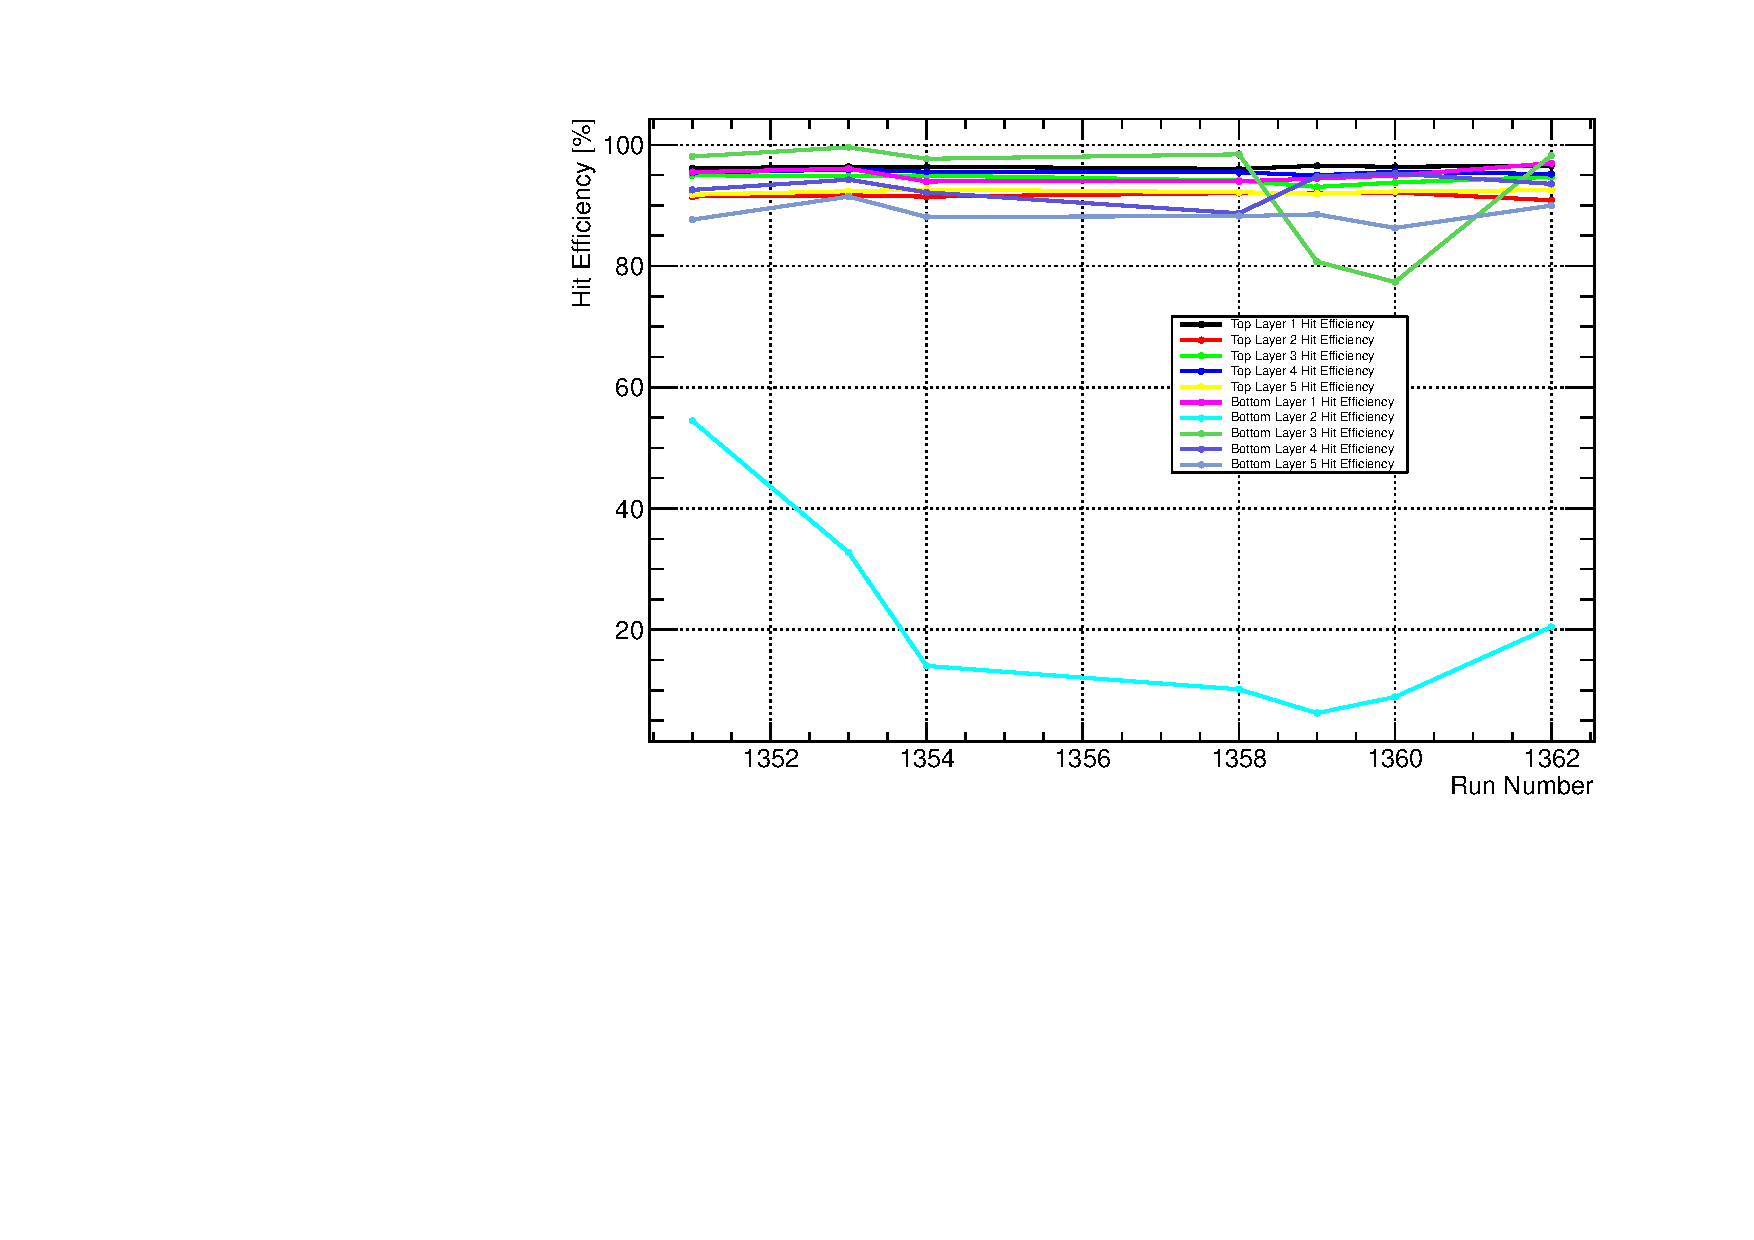
\includegraphics[width=0.98\textwidth]{test2012/svtperformance/trk_performance/hit_efficiency_vs_rn.pdf}
        \caption{} 
	\label{fig:hit_efficiency}
    \end{center}
\end{figure}
from the fit. If the track was found to lie within the sensitive volume
of the layer, a search for a stereo hit within the layer acceptance was 
conducted.  The hit efficiency was then determined as
\[
    \varepsilon_{\mbox{hit efficiency}} = \frac{\mbox{Tracks with hit on missing layer}}
                                            {\mbox{Tracks within layer acceptance}} \times 100 \%
\]
The hit efficiencies per layer were calculated using all dedicated runs. As 
can be seen from Figure~\ref{fig:hit_efficiency}, the average hit efficiency
per layer, excluding all known bad Si sensors, was found to be greater than
90\%.
% The single hit efficiencies need to be updated to reflect changes that were 
% made to the tracking code

The efficiency of the tracking algorithm was also studied and is shown on 
Figure~\ref{fig:trk_efficiency}.
\begin{figure}[h]
    \begin{center}
        % TODO: Need to update the plot so that Layer 2 on the bottom doesn't 
        % look terrible
    	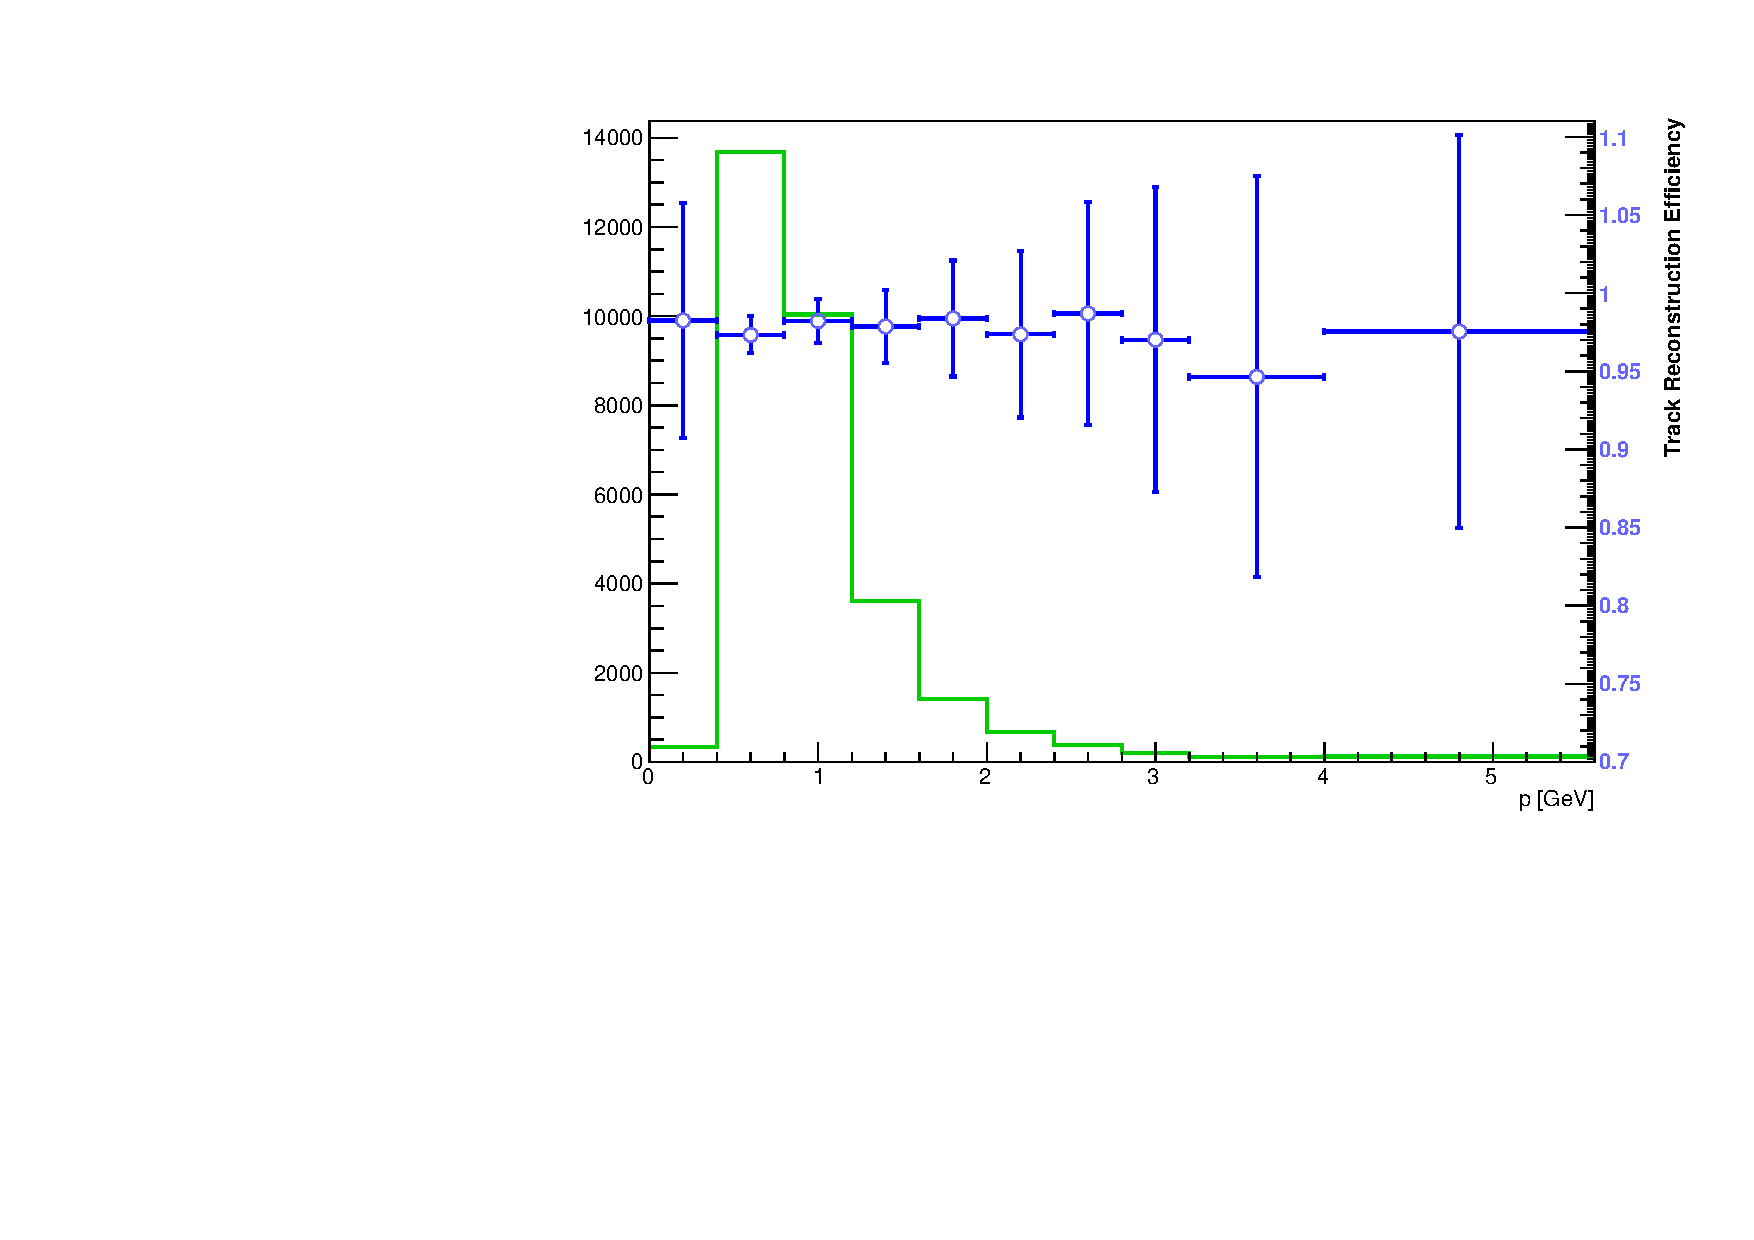
\includegraphics[width=0.98\textwidth]{test2012/svtperformance/trk_performance/track_reco_efficiency.pdf}
        \caption{} 
	\label{fig:trk_efficiency}
    \end{center}
\end{figure}
